\chapter{Экспериментальный раздел}

\section{Описание эксперимента}

Целью эксперимента является оценка изменения времени выполнения запросов на стороне БД в зависимости от наличия индексирования.

Эксперимент проводился над таблицами Users и Participants созданной базы данных.

В ходе эксперимента было исследовано влияние скорость выполнения следующих запросов к базе данных:
\begin{enumerate}
    \item select * from Participants where rating < 100.
    \item select * from Users where login = 'culturedToucan5'.
\end{enumerate}


В первом случае запрашивалась информация о всех пользователях с рейтингом меньше 100 (возвращалось около 1\% пользователей из БД). Во втором -- информация о пользователе с именем пользователя <<$culturedToucan5$>> В обоих случаях тестирование проводилось на таблицах с различным числом записей: от 10 000 до 1 000 000. Кроме того, было исследовано время индексирования таблицы и время вставки 10000 записей в проиндексированную и неиндексированную таблицы. Время выполнения каждого из запросов замерялось 20 раз, отбрасывались минимальное и максимальное значения, а затем бралось среднее арифметическое.

Построение индекса проводилось над полями rating и login для соответствующих таблиц. Индексирование проводилось при помощи алгоритма B-Tree, являющимся стандартным в PostgreSQL. Данный алгоритм позволяет ускорить выполнение запросов, использующих операции $\leq, <, =, >, \geq$ \cite{postgres_index}. 

База данных была запущена на ПК со следующими характеристиками:
\begin{itemize}
    \item RAM: 8 Гбайт DDR4;
    \item ЦПУ: AMD Ryzen 5 3500U \cite{amd};
    \item ОС: Ubuntu 20.04 \cite{ubuntu}.
    \end{itemize}

При проведении тестирования на ПК были запущены только сервисы ОС, среда разработки и база данных. Во время тестирования ПК был подключен к сети электропитания.

Полученные данные продемонстрированы на рисунках \ref{indexing_both} - \ref{insertion_time_username}.


\subsection{Запрос №1}

\begin{figure}[H]
	\begin{center}
		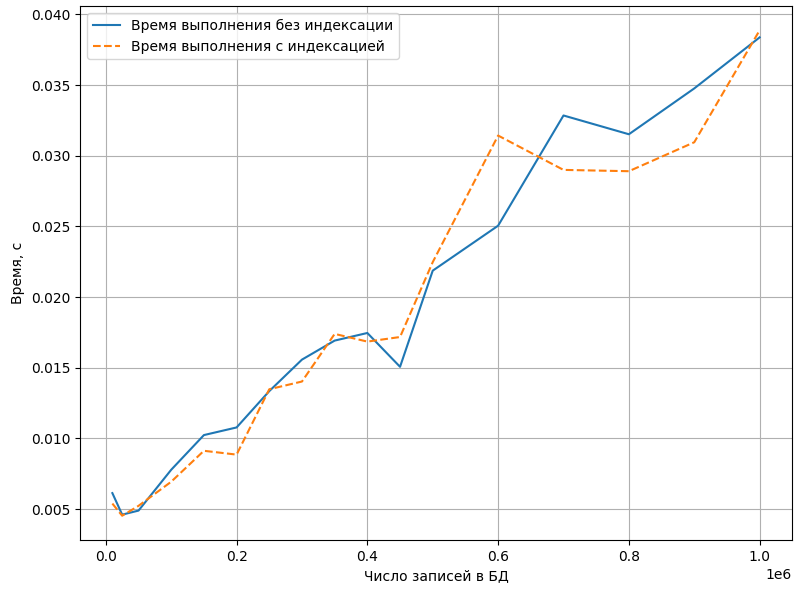
\includegraphics[page=1,scale=0.8]{assets/indexing_both.png}
	\end{center}
	\caption{Время выполнения запросов с индексацией и без}
	\label{indexing_both}
\end{figure}

\begin{figure}[H]
	\begin{center}
		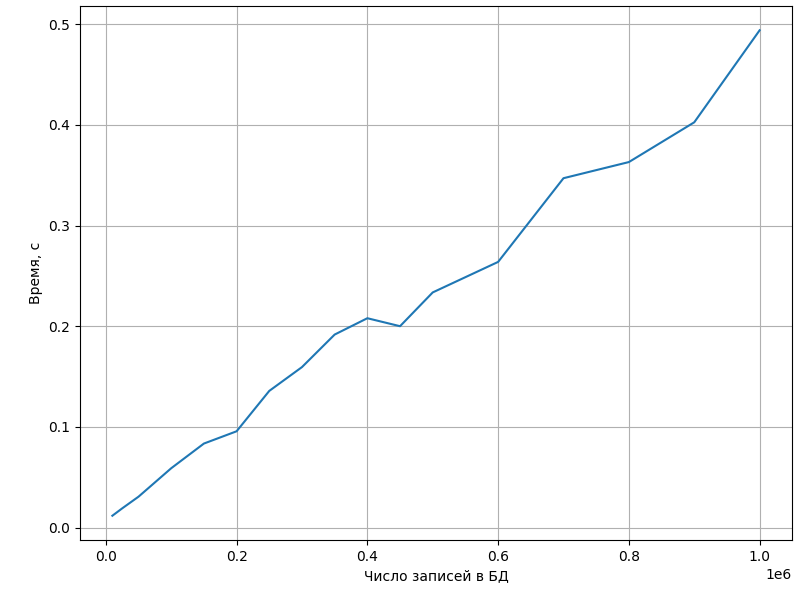
\includegraphics[page=1,scale=0.8]{assets/indexing_time.png}
	\end{center}
	\caption{Время выполнения индексации}
	\label{indexing_time}
\end{figure}

\begin{figure}[H]
	\begin{center}
		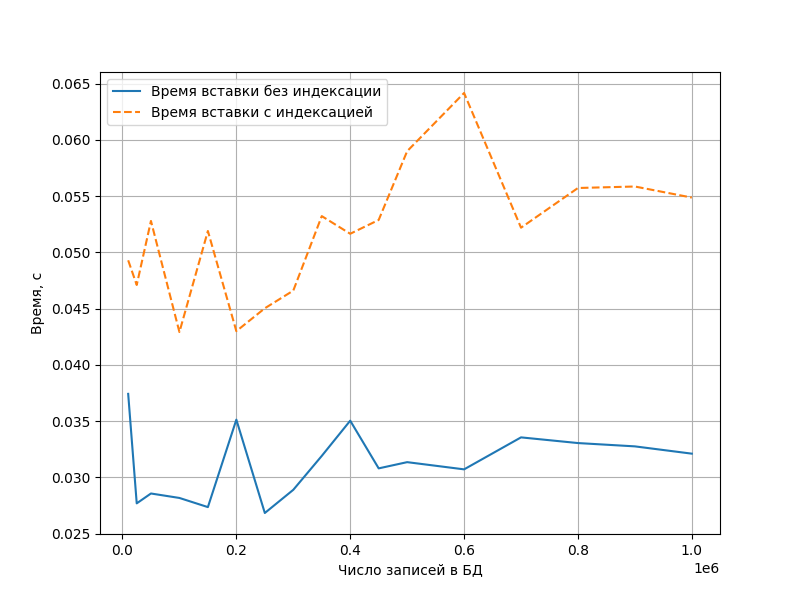
\includegraphics[page=1,scale=0.8]{assets/insertion_time.png}
	\end{center}
	\caption{Время вставки 10000 записей в таблицу}
	\label{insertion_time}
\end{figure}

По полученным данным нельзя сказать, что индексация оказала заметное воздействие на время выполнения запросов. Время индексации таблицы составило до 0.5 секунд (при 1 000 000 записей). Более того, время вставки в проиндексированную таблицу возросло в 1.5 - 2 раза по сравнению с неиндексированной таблицей.

\subsection{Запрос №2}

\begin{figure}[H]
	\begin{center}
		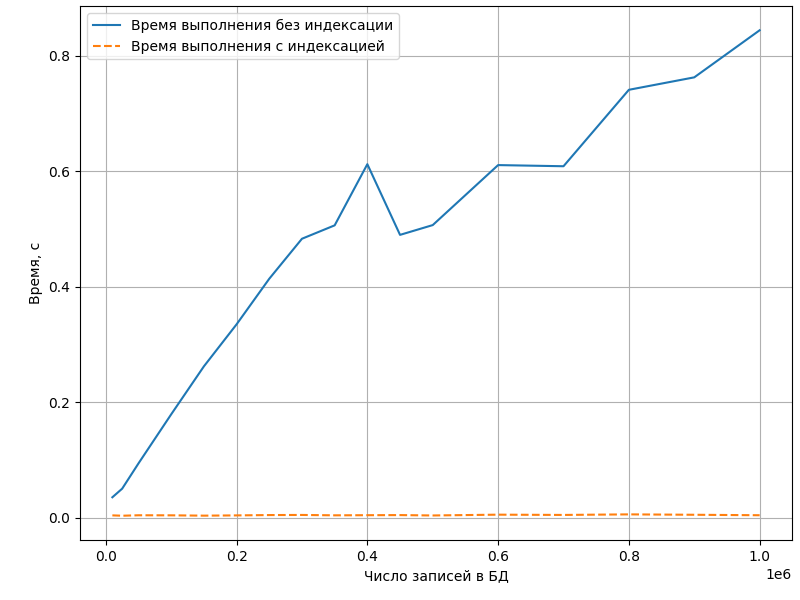
\includegraphics[page=1,scale=0.8]{assets/indexing_both_username.png}
	\end{center}
	\caption{Время выполнения запросов с индексацией и без}
	\label{indexing_both_username}
\end{figure}

\begin{figure}[H]
	\begin{center}
		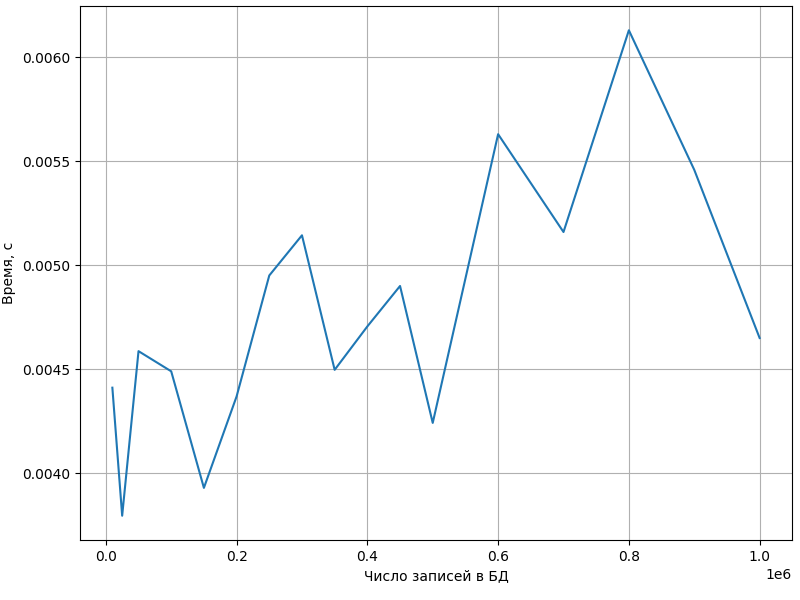
\includegraphics[page=1,scale=0.8]{assets/indexing_separate_username.png}
	\end{center}
	\caption{Время выполнения запросов с индексацией}
	\label{indexing_both_username}
\end{figure}


\begin{figure}[H]
	\begin{center}
		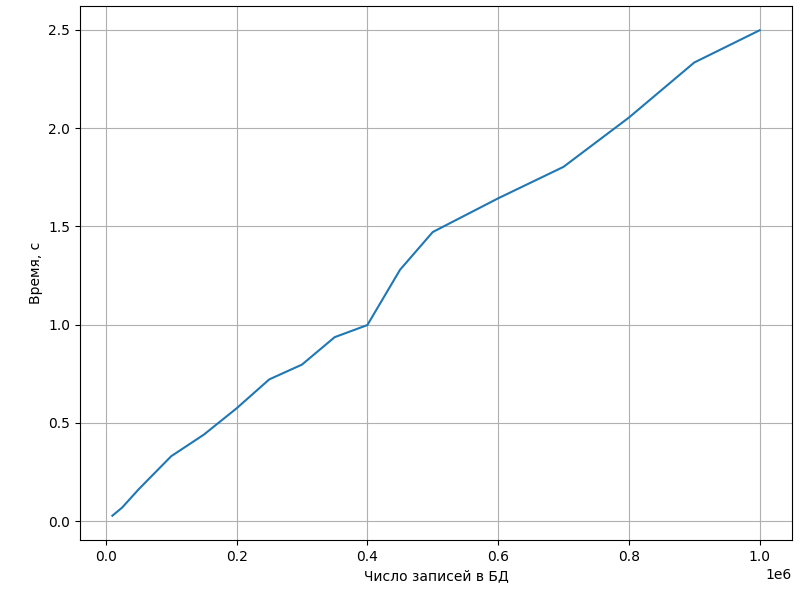
\includegraphics[page=1,scale=0.8]{assets/indexing_time_username.png}
	\end{center}
	\caption{Время выполнения индексации}
	\label{indexing_time_username}
\end{figure}

\begin{figure}[H]
	\begin{center}
		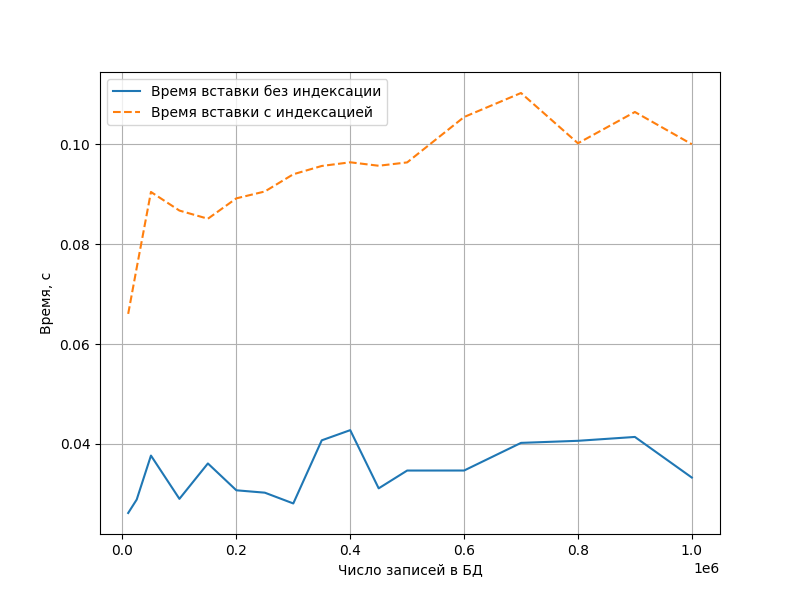
\includegraphics[page=1,scale=0.8]{assets/insertion_time_username.png}
	\end{center}
	\caption{Время вставки 10000 записей в таблицу}
	\label{insertion_time_username}
\end{figure}

В данном случае индексация позволила многократно (в 100-200 раз) сократить время выполнения запроса. Однако вместе с тем время индексации таблицы увеличилось до 2.5 с (при 1 000 000 записей) и возросло время вставки в таблицу (в 2 - 3 раза).

\section{Вывод из раздела}
В результате эксперимента обнаружено, что индексация способно многократно (по полученным данным до 200 раз) ускорить выполнение запросов к базе данных, однако имеет несколько недостатков: оно способно оказать воздействие на время выполнения запросов только при использовании уникальных для пользователя данных, увеличивает время массовой вставки в таблицу в 1,5 - 3 раза и построение индекса над таблицей также занимает время.
